


\section{Effect of other wave condition}
\label{sec: WC2 moving}

The effect of Wave Condition 2, with wave height of 9 meters and a peak period of 10.4 seconds, is studied in this section. 


\subsection{Approach}

The exact same deisgn space is used as in the first design iteration of Wave Condition 1, so also the same boundaries as shown in table \ref{tab: boundaries DI1 moving} apply.

\subsection{Correlation}
% \begin{figure}[h]
%     \centering
%     \begin{subfigure}[b]{0.30\textwidth}  
%         \centering 
%         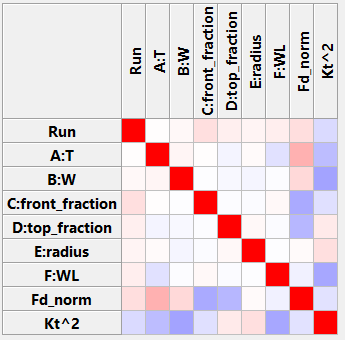
\includegraphics[width=\linewidth]{figures/ComFLOW/Results moving/DI1/H9/correlation_H9.png}
%         \caption[]%
%         {{\small Correlation between factors and responses}}    
%         \label{fig: correlation DI1 captive}
%     \end{subfigure}
    
%     \centering
%     \begin{subfigure}[b]{0.49\textwidth}
%         \centering
%         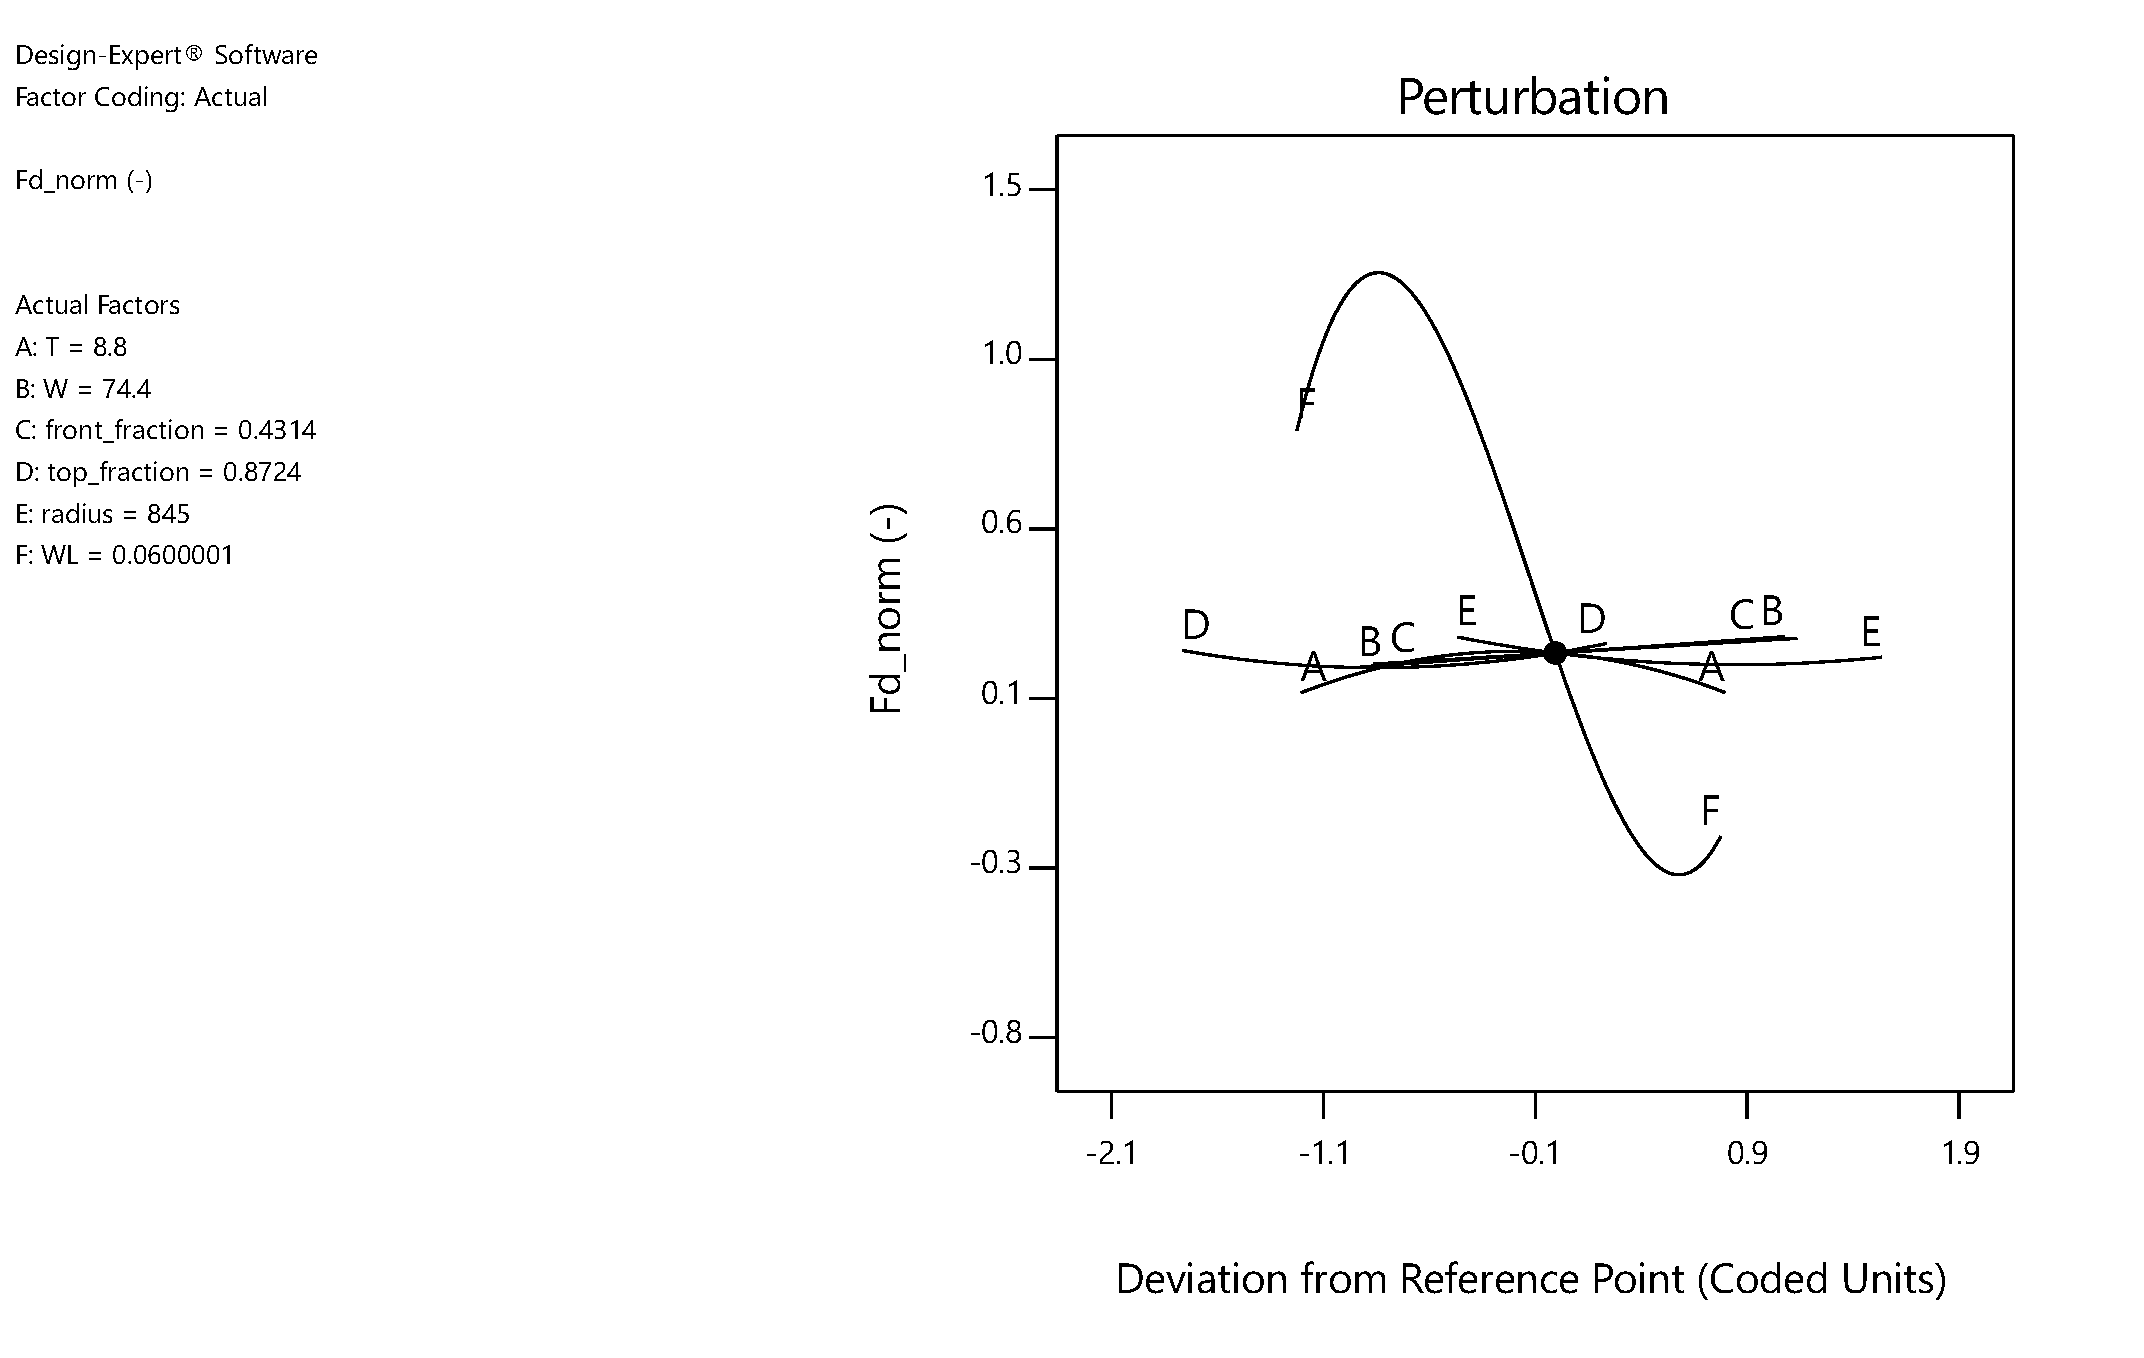
\includegraphics[width=\linewidth]{figures/ComFLOW/Results DI1/perturbation R1.pdf}
%         \caption[]%
%         {{\small Perturbation Response 1: Mean wave drift force}}    
%         \label{fig: perturbation R1 DI1 captive}
%     \end{subfigure}
%     \hfill
%     \begin{subfigure}[b]{0.49\textwidth}  
%         \centering 
%         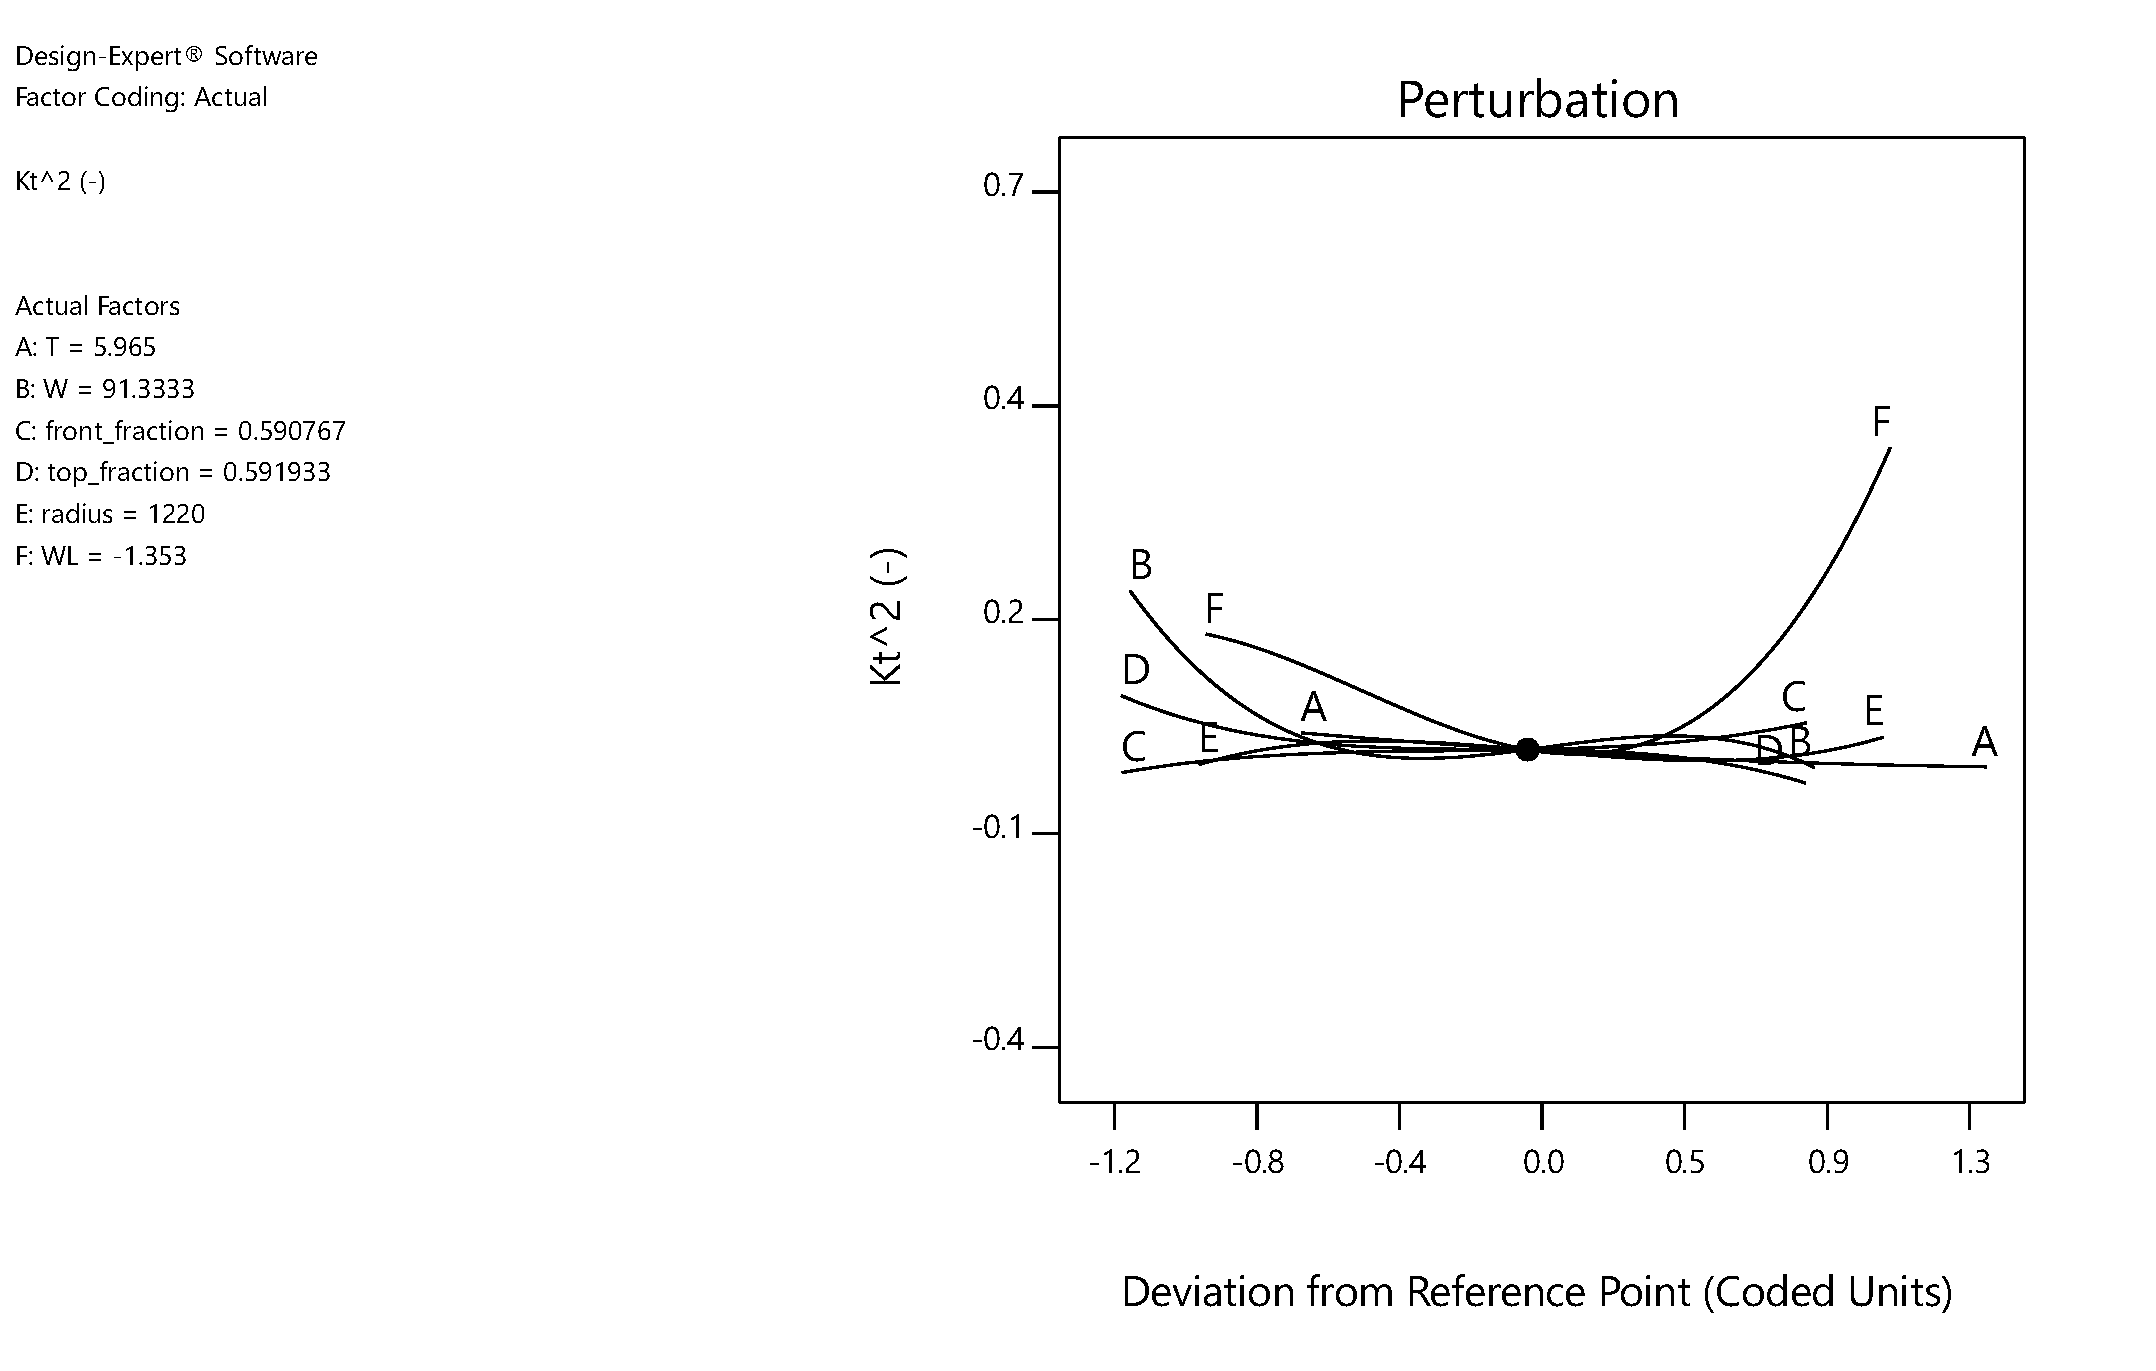
\includegraphics[width=\linewidth]{figures/ComFLOW/Results DI1/perturbation R2.pdf}
%         \caption[]%
%         {{\small Perturbation Response 2: Wave transmission coefficient}}    
%         \label{fig: perturbation R2 DI1 captive}
%     \end{subfigure}



%     \caption{}
%     \label{fig: }
% \end{figure}


Figure \ref{fig: Fd_norm_VS_top_bw_with_Kt} shows the same trend as observed in the \acrfull{cdo} is still visible, but the correlation is weaker. 

\begin{figure}[h]
    \centering
    \begin{subfigure}[b]{0.49\textwidth}
        \centering
        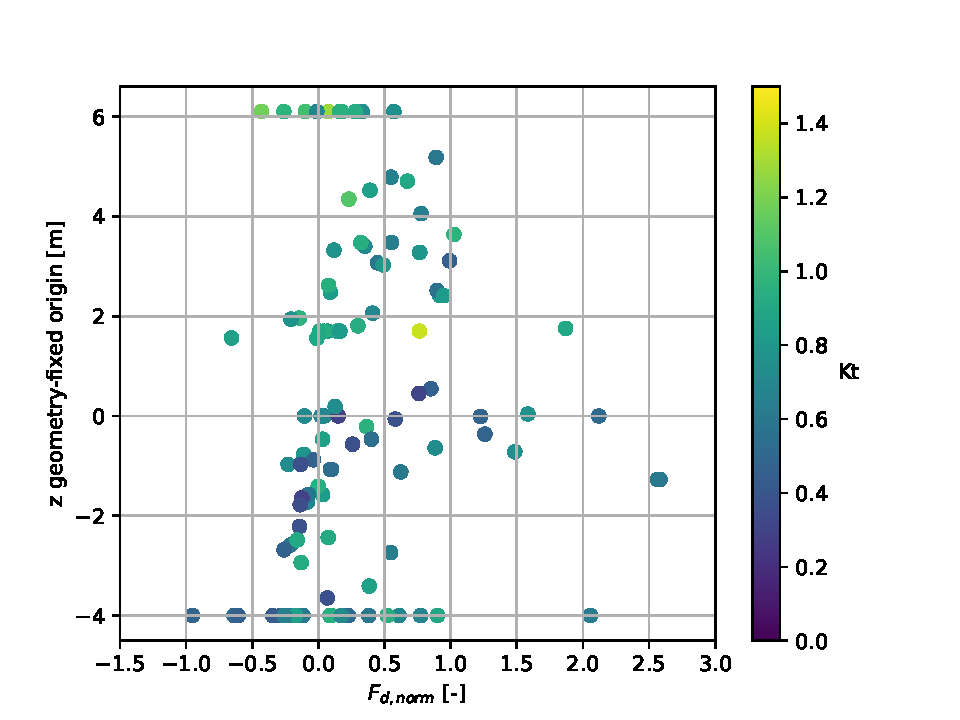
\includegraphics[width=\linewidth]{figures/ComFLOW/Results moving/DI1/H9/Fd_norm_VS_top_bw_with_Kt.pdf}
        \caption[]%
        {{\small }}    
        \label{fig: Fd_norm_VS_top_bw_with_Kt}
    \end{subfigure}
    \hfill
    \begin{subfigure}[b]{0.49\textwidth}  
        \centering 
        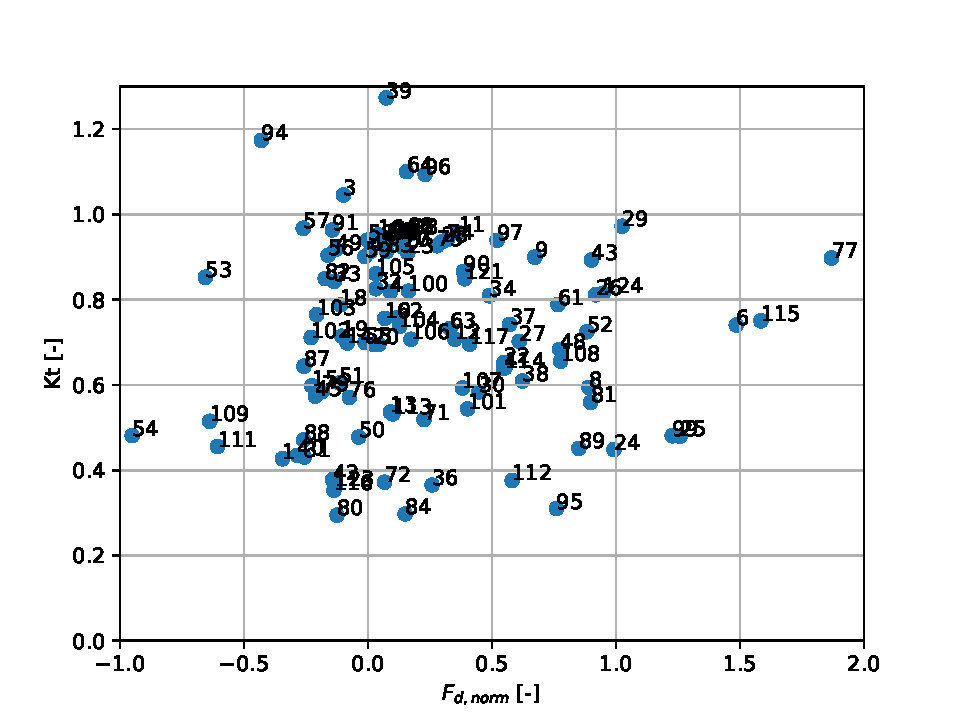
\includegraphics[width=\linewidth]{figures/ComFLOW/Results moving/DI1/H9/Fd_norm_VS_Kt.pdf}
        \caption[]%
        {{\small }}    
        \label{fig:  Fd_norm vs Kt}
    \end{subfigure}
    
    \caption{}
    \label{fig: }
\end{figure}



\subsection{Design Optima}




%%%%%%%%%%%%%%%%%%%%%%%%%%%%%%%%%%%%%%%%%%%%%%%%%%%%%%%%%%%%%%%%%%%%%%%%%%%%%%%%%%%%
\subsubsection{Based on minimal mean wave drift force}


All optima found in order to reach the minimal mean wave drift force cross the waterline and are having a small draught. Also, they converged to the largest width, which was not the case for the \acrfull{cdo} with the same wave condition. 


\begin{table}[H]
\centering
\scalebox{0.65}{
\begin{tabular}{@{}ccccccccccc@{}}
\toprule
configuration & T        & W        & front\_fraction & top\_fraction & radius   & WL & $F_{d,norm,DoE}$ & $K_{t,DoE}^2$  & $F_{d,norm,ComFLOW}$  & $K_{t,ComFLOW}^2$      \\ \midrule
1  & 6.92 & 149.73 & 0.75 & 0.90 & 1722.45 & -6.05 & -1.50 & 1.21 &  &  \\
2  & 5.44 & 147.84 & 0.16 & 0.93 & 820.01  & -4.24 & -1.53 & 1.16 &  &  \\
3  & 2.52 & 149.60 & 0.06 & 0.95 & 501.78  & -1.72 & -1.52 & 1.05 &  &  \\
4  & 6.48 & 149.54 & 0.35 & 0.97 & 868.08  & -4.71 & -1.66 & 1.15 &  &  \\
5  & 6.83 & 142.78 & 0.26 & 0.95 & 1234.32 & -5.24 & -1.63 & 1.11 &  &  \\
6  & 2.73 & 148.82 & 0.02 & 0.98 & 1014.88 & -1.93 & -1.53 & 1.06 &  &  \\
7  & 6.77 & 131.02 & 0.14 & 0.99 & 1371.67 & -5.74 & -1.71 & 1.04 &  &  \\
8  & 4.72 & 149.79 & 0.11 & 0.99 & 1437.92 & -3.87 & -1.81 & 1.19 &  &  \\
9  & 4.70 & 149.82 & 0.07 & 0.97 & 549.02  & -3.09 & -1.50 & 1.11 &  &  \\
10 & 2.53 & 149.85 & 0.07 & 0.98 & 692.33  & -1.72 & -1.54 & 1.05 &  & \\ \bottomrule
\end{tabular}
}
\caption{Parameters optimal breakwaters based on minimal mean wave drift force}
\label{tab: params design iteration 1 moving br 1to10 mean wave drift force}
\end{table}


\begin{figure}[h]
    \centering
    \begin{subfigure}[b]{0.49\textwidth}
        \centering
        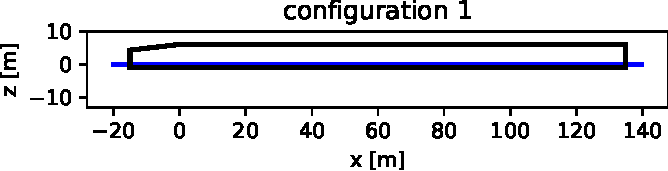
\includegraphics[width=\textwidth]{figures/ComFLOW/Breakwater Geometries/DI1 moving/WC2/optima_Fd/breakwater_geometry1.pdf}
        \caption[]%
        {{\small}}    
        \label{fig: opt breakwater 1 moving fd WC2}
    \end{subfigure}
    \hfill
    \begin{subfigure}[b]{0.49\textwidth}  
        \centering 
        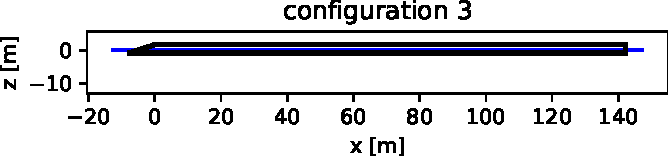
\includegraphics[width=\textwidth]{figures/ComFLOW/Breakwater Geometries/DI1 moving/WC2/optima_Fd/breakwater_geometry3.pdf}
        \caption[]%
        {{\small}}    
        \label{fig: opt breakwater 3 moving fd WC2}
    \end{subfigure}
    
    \caption{The two most optimal breakwaters based on the mean wave drift force}
    \label{fig: two most optimal breakwaters moving fd WC2}
\end{figure}




%%%%%%%%%%%%%%%%%%%%%%%%%%%%%%%%%%%%%%%%%%%%%%%%%%%%%%%%%%%%%%%%%%%%%%%%%%%%%%%%%%%%
\subsubsection{Based on minimal transmission coefficient}

Here the breakwaters converged to almost the maximum depth, but a smaller width and are placed close to the waterline. 

\begin{table}[H]
\centering
\scalebox{0.65}{
\begin{tabular}{@{}ccccccccccc@{}}
\toprule
configuration & T        & W        & front\_fraction & top\_fraction & radius   & WL & $F_{d,norm,DoE}$ & $K_{t,DoE}^2$  & $F_{d,norm,ComFLOW}$  & $K_{t,ComFLOW}^2$      \\ \midrule
1  & 12.69 & 91.15  & 0.90 & 0.01 & 1448.88 & 0.08  & 1.12 & 0.00  & 0.33 & 0.067 \\
2  & 12.92 & 88.66  & 0.81 & 0.01 & 936.09  & 0.03  & 1.34 & 0.00  & 0.46 & 0.070 \\
3  & 12.83 & 95.19  & 0.92 & 0.02 & 1778.81 & -0.10 & 1.27 & 0.00  &  &  \\
4  & 12.87 & 100.64 & 0.98 & 0.03 & 1123.05 & -0.08 & 0.95 & 0.00  &  &  \\
5  & 12.63 & 87.38  & 0.99 & 0.01 & 1885.36 & -0.12 & 0.87 & -0.01 &  &  \\
6  & 12.60 & 88.78  & 0.87 & 0.01 & 1999.34 & -0.40 & 1.37 & 0.00  &  &  \\
7  & 12.74 & 91.60  & 0.99 & 0.03 & 1102.75 & 0.21  & 0.72 & 0.00  &  &  \\
8  & 12.87 & 88.38  & 0.98 & 0.04 & 1995.47 & 0.07  & 1.01 & 0.00  &  &  \\
9  & 12.92 & 92.69  & 0.98 & 0.06 & 1184.21 & -0.04 & 0.90 & 0.00  &  &  \\
10 & 12.88 & 88.71  & 0.98 & 0.05 & 1910.57 & -0.06 & 1.03 & 0.00  &  & \\ \bottomrule
\end{tabular}
}
\caption{Parameters optimal breakwaters based on minimal transmission coefficient}
\label{tab: params design iteration 1 moving br 1to10 transmission}
\end{table}


\begin{figure}[h]

        \centering
        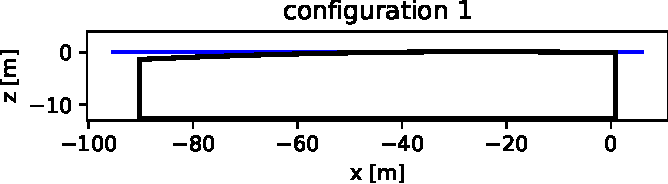
\includegraphics[width=0.49\textwidth]{figures/ComFLOW/Breakwater Geometries/DI1 moving/WC2/optima_Kt/breakwater_geometry1.pdf}

    \caption{The most optimal breakwater based on the transmission coefficient}
    \label{fig: two most optimal breakwaters moving kt WC2}
\end{figure}

